%chktex-file 36
%chktex-file 23
%chktex-file 10
%chktex-file 17
%chktex-file 9
\documentclass[computationalMathematics.tex]{subfiles}

\begin{document}

%%%%%%%%%%%%%%~~~~~~~~~~~~~~~~~~~~~~~~~~~~~~~~~~~~~~~~%%%%%%%%%%%%%%%
\section{20th of September 2018 --- F. Poloni}
%%%%%%%%%%%%%%~~~~~~~~~~~~~~~~~~~~~~~~~~~~~~~~~~~~~~~~%%%%%%%%%%%%%%%

\subsection{A warm up}
Before starting here is a small recap
\begin{itemize}
    \item \textbf{Vector-Scalar product}:\\
      Let $x \in \R^n$ and $\lambda \in \R$ we call \textbf{multiple} of vector $x$ the following:\\ $$\lambda x = x \lambda = \begin{pmatrix}\lambda x_1\\
        \vdots\\
        \lambda x_n\\
      \end{pmatrix}$$.
    
    \item \textbf{Vector-Vector product}:\\
     Let $x, y \in \R^n$. The product between those two vectors is computed as follows $\tr{x} y = \sum\limits_{i=1}^n x_i y_i$ and $\tr{x}y \in \R$.
     
     \item \textbf{Scalar-Matrix product}:\\
      Let $A \in \R^{n\times m}$ and $\lambda \in \R$ we call the \textbf{scalar-matrix product} the following:\\ $$\lambda A = A \lambda = 
      \begin{pmatrix}
        \lambda A_{11}  & \lambda A_{12} & ...\\
        \lambda A_{21}  & \lambda A_{22} & ... \\
        \vdots  &\vdots & \ddots \\
      \end{pmatrix}$$.
     
     \item \textbf{Matrix-Vector product}:\\
        Given a matrix $A \in M(n, m, \R)$ and a vector $v \in \R^m$ the \textbf{matrix-vector product} $A v = w \in \R^n$ is computed as follows:
        \[
          w = Av = \begin{pmatrix}
          A_1 v\\
          A_2 v\\
          \vdots\\
          A_m v\\
          \end{pmatrix}, \, 
          w_i = \sum\limits_{j=1}^m A_{ij} v_j
        \]
        This is the simple way, just a row-by-column vector product, the computational complexity of this operation is $O(n^2)$.\\
        The smart way to compute it: \textbf{linear combinations} of columns of A, e.g.:\\
        $$
            \begin{pmatrix}
                      A_{11} & A_{12} & A_{13}\\
                      A_{21} & A_{22} & A_{23}\\
                      A_{31} & A_{32} & A_{33}\\
                      A_{41} & A_{42} & A_{43}
            \end{pmatrix}
            \begin{pmatrix}
                      v_1\\
                      v_2\\
                      v_3
            \end{pmatrix} =
            \begin{pmatrix}
                      w_1\\
                      w_2\\
                      w_3
            \end{pmatrix}
        $$
        with \textbf{linear combinations} we have:
        $$
        \begin{pmatrix}
                A_{11}\\
                A_{21}\\
                A_{31}\\
                A_{41}
        \end{pmatrix}v_1 +
        \begin{pmatrix}
                A_{12}\\
                A_{22}\\
                A_{32}\\
                A_{42}
        \end{pmatrix}v_2 + 
        \begin{pmatrix}
                A_{13}\\
                A_{23}\\
                A_{33}\\
                A_{43}
        \end{pmatrix}v_3 =
        \begin{pmatrix}
                  w_1\\
                  w_2\\
                  w_3\\
                  w_4
        \end{pmatrix}
        $$
  \item \textbf{Matrix-Matrix Product}:\\
        Given two matrices $A \in \R^{n\times m}$ and $B \in \R^{m\times k}$ we call \textbf{matrix-matrix product} the following:
        $C=AB$ such that $C_{ij} = A_i B^j$, where $\tr{A_i} \in \R^m$ is the $i$-th row of $A$, $B^i$ is the $i$-th column of $B$ ($B^i \in \R^m$) and $C \in M(n, k, \R)$. Notice that this product is \textbf{not commutative}: $AB \neq BA$ might not even make sense dimension-wise.
        
        Computational Cost: multiplying $m \times n$ and $n \times p$ requires $m(2n - 1)p$ floating point operations (flops) and two matrix, A and B, are both $ n \times n$ is $O(n^2)$. Forget about fancier algorithms (e.g. Strassen)
        
        \begin{myframe}{\bf Order of operations}
        Usual algebra properties hold, e.g.: A(B + C) = AB + AC, A(BC) = (AB)C, etc... \\
        Parenthesization matters a lot: if $A, B \in \R^{n \times n }, \, v \in \R^n$, then $(AB)v$ costs $O(n^3)$, but $A(Bv)$ costs $O(n^2)$.
        Programming languages usually do not rearrange parentheses to help.
        \end{myframe}

     \item \textbf{Image} of a matrix $A$ ($\text{Im}(A)$):  the set of vectors that can    be obtained multiplying $A$ by any vector in the domain of $A$.

     \item \textbf{Kernel} of a matrix $A$ ($\ker(A)$):  the set of vectors $w$ in its domain such that $Aw=0$.

     \item Given a matrix $A \in M(n, \R)$ we call \textbf{inverse} of $A$ the matrix $\inv{A}$ such that:
         $$\inv{A} A = A \inv{A} = I_{n} =
         \begin{pmatrix}
                1\\
                & 1\\
                & & 1\\
                & & & \ddots\\
                & & & & 1
         \end{pmatrix}$$
         The \textbf{inverse of a product} (shoe-sock identity) is $\inv{(A B)} = \inv{B} \inv{A}$. Notice that this identity holds only for square matrices.

     \item The \textbf{transpose} of a matrix $A \in M(n, m, \R)$ is $\tr{A}$ such that $\tr{A}_{ij} = A_{ji}$. The \textbf{transpose of a product} (shoe-sock identity) is $\tr{(A B)} = \tr{B} \tr{A}$. ( This identity holds for square and rectangular matrices)

\end{itemize} 

\begin{definition}
  \textbf{General linear group (GL)}: the general linear group of degree n is the set of $n\times n$ invertible matrices, together with the operation of ordinary matrix multiplication
\end{definition}

\begin{proposition}
  Let $A \in GL(n, \R)$ (aka $A$ is a real square matrix of size $n$ and invertible), $B, C \in M(n, m, \R)$ and we have the product $AB = AC$. If there is a matrix $M$ such that $MA = I$: 
  $$(MA)B = (MA)C \Longleftrightarrow B=C, \,\, M = A^{-1}$$.
\end{proposition}
\noindent So $AB = AC$ does not usually imply $B = C$, $A$ must be invertible!\\

\begin{myframe}{\bf Row and column vectors notation}
        $$v =   \begin{pmatrix}
                    4\\
                    5\\
                    6
                \end{pmatrix},\,
          v^T = \begin{pmatrix}
                    4 & 5 & 6
          \end{pmatrix}$$
          $v$ is a column vector in $\R^3$ (or a matrix in $\R^{3 \times 1}$) and $v^T$ is a row vector (or a matrix in $\R^{1\times 3}$).
\end{myframe}

\begin{definition}
  \textbf{Basis}: a set $B$ of elements (vectors) in a vector space $V$ is called a \textbf{basis}, if every element of $V$ may be written in a unique way as a (finite) linear combination of elements of $B$. The coefficients of this linear combination are referred to as components or coordinates on $B$ of the vector. The elements of a basis are called basis vectors.
\end{definition}
\noindent\textbf{Canonical basis}: $w = w_1e_1 + w_2e_2 + w_3e_3 + w_4e_4, \,$ e.g. for $m = 4$\\
$$  e_1 = \begin{pmatrix} 1\\ 0\\ 0\\ 0 \end{pmatrix}\, , \,
    e_2 = \begin{pmatrix} 0\\ 1\\ 0\\ 0 \end{pmatrix}\, , \,
    e_3 = \begin{pmatrix} 0\\ 0\\ 1\\ 0 \end{pmatrix}\, , \,
    e_4 = \begin{pmatrix} 0\\ 0\\ 0\\ 1 \end{pmatrix}$$
The powerful idea behind linear algebra: many relations are true
regardless of the basis we use. E.g. $w$, $v$ and $w + v$ in two different bases.
\begin{figure}[H]
    \centering
    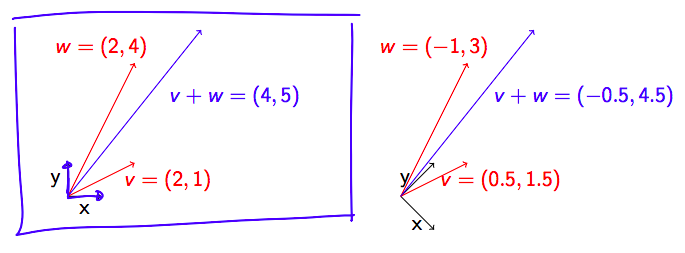
\includegraphics[scale=0.45]{pics/20sett/3.png}
    \label{fig:20sett1}
\end{figure}

\subsection{Solving Linear Systems}
The objective of this course, for the part concerning numerical methods, is solving linear systems efficiently.

\begin{definition}[Linear system]
  Let $A \in M(n, m, \R)$, $b \in \R^n$ and $x \in \R^m$. We term \textbf{linear system} the following:

  \[
Ax = b
  \]
\end{definition}

\noindent Our goal is to approximate such vector $x$, hence resulting in solving a minimum problem:

\[
  \min\limits \norm{Ax - b}
\]

If we have a square and invertible A matrix solve a linear systems means: find coordinates $x_1, \dots , x_m$ needed to write $b$ as linear combinations of the columns of (square) $A\in\R^{m\times m}$ and in this case, the solution is given by: $x = A^{-1}b$. \\
\textbf{Warning}: this is not the best way to solve a linear system on a computer!\\

\syntax{Notice that the machine precision is $10^{-16}$, so we should pay attention when making computations, since we may incur in some error (proportional to the size of the operands).

In Matlab a matrix is written as \texttt{A=[1, 2, 3; 4, 5, 6];}, where \texttt{[1, 2, 3]} is the first row of the matrix A.

The transpose of a matrix or a vector is denoted by \texttt{A'}.

The inverse of a square matrix is denoted by \texttt{inv(A)}.

If we are interested in only a part of our matrix \texttt{A} we may write \texttt{A[1:2, 1:3]} and obtain only the rows of \texttt{A} that go from $1$ to $2$ and those columns from $1$ to $3$.
}



\begin{definition}[Block multiplications]
  Let $A \in M(n,m, \R)$ and let $B \in M(m, k, \R)$. We can compute the result of a block of the matrix $AB$ as the product of the two blocks in $A$ and $B$ in the corresponding position.
\begin{figure}[H]
    \centering
    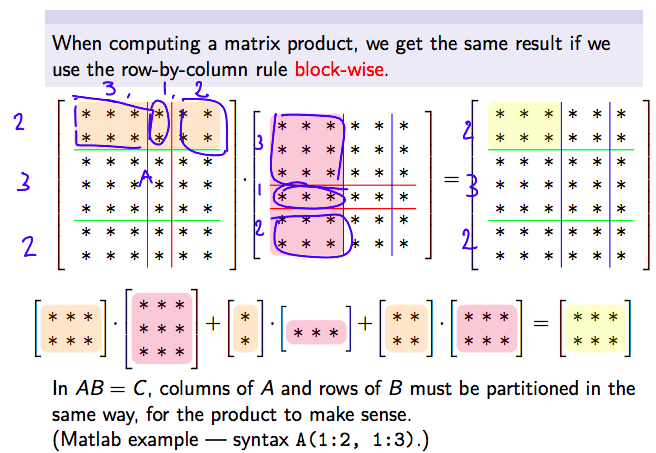
\includegraphics[scale=0.40]{pics/20sett/2.png}
    \label{fig:20sett2}
\end{figure}
\end{definition}


\textbf{Note}: Block operations usually give better performance: one
matrix-matrix product performs faster than n matrix-vector
products (even if they have the same number of flops).
This is one of the reasons why library calls usually perform better
than hand-coded loops (Blas/Lapack).

\begin{proposition}[Block triangular matrices]
  Let $M \in M(n, m, \R)$ and $B \in M(m, k, \R)$ such that they are \textbf{block triangular}.
  Their product is a block triangular matrix as well, block triangular matrices
are closed under products:
  $$M B 
  = \begin{pmatrix}
    A & B\\
    0 & C
  \end{pmatrix}
  \begin{pmatrix}
    D & E\\
    0 & F
  \end{pmatrix}
  = 
  \begin{pmatrix}
    AD & AE + BF\\
    0 & CF
  \end{pmatrix}$$
\end{proposition}

\begin{proposition}[Properties of triangular matrices]~\\
    Let M be a block triangular matrix, with all $A_{ii}$ square
    $$M 
      = \begin{pmatrix}
        A_{11}  & A_{12} & ... & A_{1k}\\
        0       & A_{22} & ... & A_{2k}\\
        \vdots  &\ddots & \ddots & \vdots\\
        0       & ... & 0 & A_{kk}
      \end{pmatrix}$$ 
    \begin{enumerate}
      \item A block triangular matrix is invertible iff all diagonal blocks $A_{ii}$ are invertible;
      \item The eigenvalues of a block triangular matrix are the union of the eigenvalues of each $A_{ii}$ block;
      \item Let $M \in GL(n, m, \R)$ such that $M= 
        \begin{pmatrix}
          A & B\\
          0 & C\\
        \end{pmatrix}$ 
       the inverse of $M$ is 
        
        $\inv{M} = 
        \begin{pmatrix}
          \inv{A} & -\inv{A}B\inv{D}\\
          0 & \inv{C}
        \end{pmatrix}$.
      \item The product of two block (upper/lower) triangular matrices
(with compatible block sizes) is still block triangular
    \end{enumerate}
  \end{proposition}

Why are we interested in block triangular matrices? They depict a situation as shown in \Cref{fig:20sett3}.
\begin{figure}[H]
    \centering
    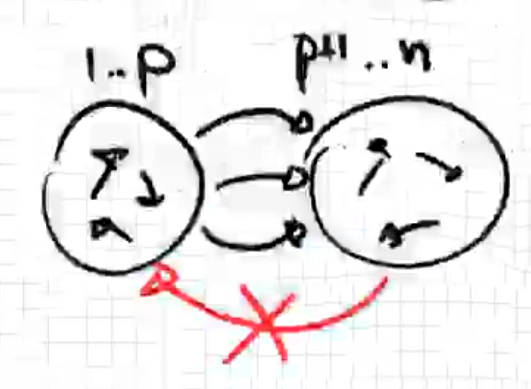
\includegraphics[scale=1]{pics/20sett/1.png}
    \caption{The adjacency matrix of a biparted graph has $0$s in its bottom left part (Matlab syntax \texttt{A[p+1:n; 1:p]=0}).}
    \label{fig:20sett3}
\end{figure}

\textbf{General principle}: matrix structures matter. Block triangular linear system has a cheaper system solution than a general system as shown in \cref{exp1:20sett}.
\begin{example}
\label{exp1:20sett}
2x2 block triangular linear system\\
$$
\begin{pmatrix}
    A & B\\
    0 & C
\end{pmatrix}*
\begin{pmatrix}
    x \\
    y 
\end{pmatrix} = 
\begin{pmatrix}
    e \\
    f 
\end{pmatrix}
$$
(Again, diagonal blocks are square and all dimensions are
compatible.)
$$
\begin{pmatrix}
    Ax + By\\
    Cy
\end{pmatrix} = 
\begin{pmatrix}
    e \\
    f 
\end{pmatrix}\implies y = \inv{C}f, x = \inv{A}(e - B\inv{C}f)
$$
$$
\begin{pmatrix}
    A & B\\
    0 & C
\end{pmatrix}^{-1} = 
\begin{pmatrix}
          \inv{A} & -\inv{A}B\inv{C}\\
          0 & \inv{C}
        \end{pmatrix}
$$
Informal idea: we can start solving from the variables in C.
\end{example}

\subsection{Orthogonality}

\begin{definition}[Norms]\label{def:20sett_norm}
  Let $x \in \R^n$. We ``measure'' their magnitude using so-called ``norms''.
  \begin{description}
    \item[{\sc Euclidean:}] $\norm{x}_2 = \tr{x} x = \sqrt{\sum\limits_{i=1}^n {x_i}^2}$;
    \item[{\sc Norm 1:}] $\norm{x}_1= \sum\limits_{i=1}^n \abs{x_i}$;
    \item[{\sc $p$-Norm:}] $\abs{x}_p = {\bigg(\sum\limits_{i=1}^n \abs{x_i}^p\bigg)}^{1/p}$;
    \item[{\sc $0$-Norm:}] $\norm{x}_0 = \abs{\{i~:~\abs{x_i} > 0\}}$;
    \item[{\sc $\infty$-Norm:}]$\norm{x}_\infty = \max\limits_{i=1, \ldots, n} \abs{x_i}$.
  \end{description}
\end{definition}

From now on in this part of th course we will refer to norm-2 only.



\begin{definition}[Orthogonal matrix]
    Let $A \in M(n, \R)$ a square matrix. $A$ is orthogonal iff:
    \begin{itemize}
        \item $\tr{A} A  = I_{n}$
        \item $A \tr{A} = I_{n}$
        \item $A^{-1} = U^T$
    \end{itemize}
  where $I_n$ is the identity matrix of size $n$ ($1$ on the diagonal, $0$ elsewhere).
\end{definition}


\end{document}


